\section{Results}
\label{sec:results}
Our experiments demonstrate the efficacy of our method in enhancing the visual representation of objects within reconstructed 3D scenes. Figure 1 (TODO FIGURE 1 IS WRONG!) shows that the output of Panoptic 3D exhibits visual artificats and irregularities, while our approach yields smooth surfaces, improving visual aesthetics. Notably, we observe sensitivity of our alignment procedure to the quality of the instance masks generated by Panoptic 3D. Although the refined objects maintain smoothness even in bad quality mask predictions, our alignment algorithm occasionally fails in unfavourable conditions, resulting in object intersections, as illustrated in \cref{fig:lim}.

\paragraph{Panoptic Reconstruction Training}

We leverage our synthesized dataset to refine the training of the panoptic reconstruction model proposed by \citet{dahnert2021panoptic}.
Initially, we pre-train the 2D encoder, depth estimation and 2D instance prediction using the ADAM optimizer \citep{kingma2014adam} using a batch size of 1 and learning rate 1e-4 for 570k iterations.

The evaluation results for our 2D model compared to the pre-trained model from \citet{dahnert2021panoptic} are presented in \cref{tab:2dresults}.
As illustrated in \cref{fig:qual_panoptic}, our approach shows performance comparable to the pre-trained model. However, it encounters challenges in generating completely clear depth results, occasionally displaying some irregularities.
Hence, we use the pre-trained version of Panoptic 3D for our remaining inference experiments. We refer to \cref{sec:future} for avenues for future work.
\begin{table}
  \centering
  \begin{tabular}{@{}lccc@{}}
    \toprule
     & Depth & Box Class. & Box Regress. \\
    \midrule
    \citet{dahnert2021panoptic} & 0.23 & 3.39 & \textbf{0.092}\\
    Ours & \textbf{0.196} & \textbf{1.3} & 0.149 \\
    \bottomrule
  \end{tabular}
  \caption{Results for joint training of the 2D encoder, depth estimation and 2D instance prediction. For depth we report the $\ell_1$ distance between the predicted and ground-truth depth maps. Additionally we report the $\ell_1$ distance for the regressed 2D boxes and a CE-loss on the box classification.  }
  \label{tab:2dresults}
\end{table}

\begin{figure}[t]
  \centering
  \begin{subfigure}[b]{0.45\linewidth}
    \centering
    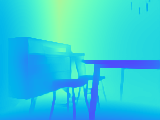
\includegraphics[width=\linewidth]{figs/depth_ours.png}
    \label{subfig:sub1}
   \vspace*{-3mm} % Adjust vertical spacing between the caption and the images
  \caption{Depth map (ours).}
  \end{subfigure}
  \hfill
  \begin{subfigure}[b]{0.45\linewidth}
    \centering
    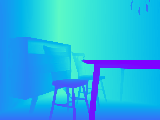
\includegraphics[width=\linewidth]{figs/depth_pan.png}
    \label{subfig:sub2}
   \vspace*{-3mm} % Adjust vertical spacing between the caption and the images
  \caption{Depth map (\citep{dahnert2021panoptic}).}
  \end{subfigure}

  \vspace{0.03\linewidth} % Adjust vertical spacing between rows of figures

  \begin{subfigure}[b]{0.45\linewidth}
    \centering
    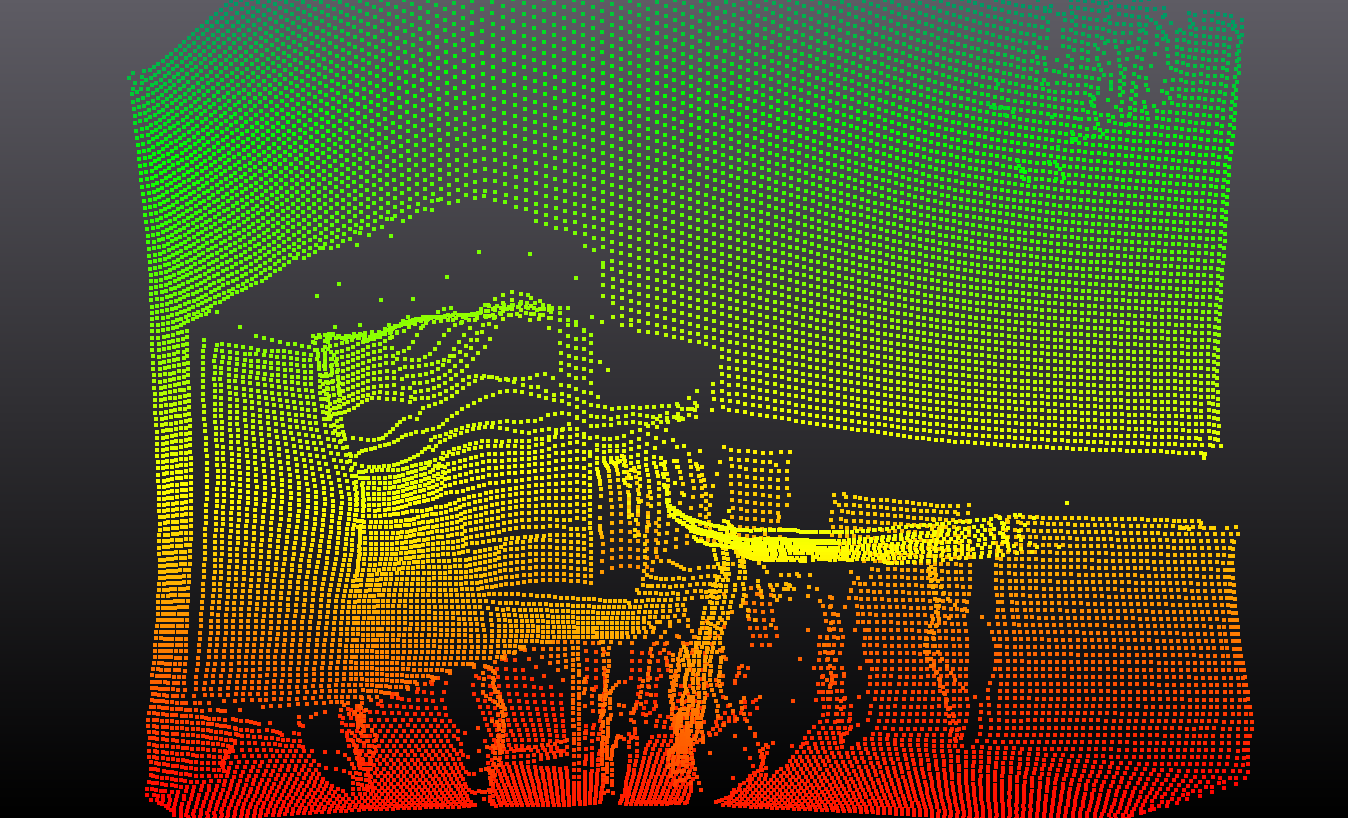
\includegraphics[width=\linewidth]{figs/depthply_ours.png}
    \label{subfig:sub3}
   \vspace*{-3mm} % Adjust vertical spacing between the caption and the images
   \caption{Geometry from depth (ours).}
  \end{subfigure}
  \hfill
  \begin{subfigure}[b]{0.45\linewidth}
    \centering
    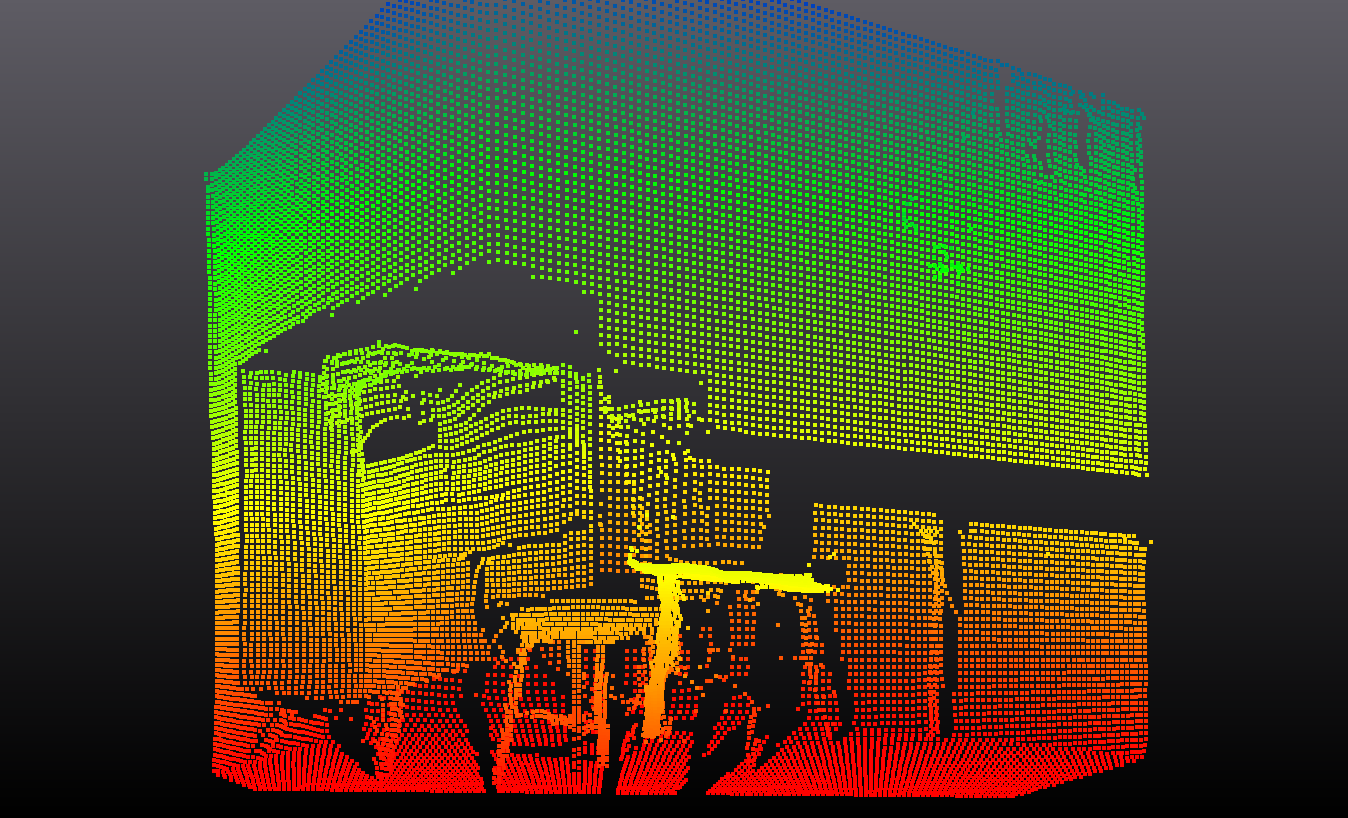
\includegraphics[width=\linewidth]{figs/depthply_pan.png}
    \label{subfig:sub4}
   \vspace*{-3mm} % Adjust vertical spacing between the caption and the images
   \caption{Geometry from depth (\citep{dahnert2021panoptic}).}
  \end{subfigure}

  \caption{2D results from the Panoptic 3D model. Our re-training results (left) vs. results from \citet{dahnert2021panoptic} (right).}
  \label{fig:qual_panoptic}
\end{figure}

\paragraph{Refined Reconstruction}

\begin{figure*}%
  \begin{subfigure}[t]{109mm}
    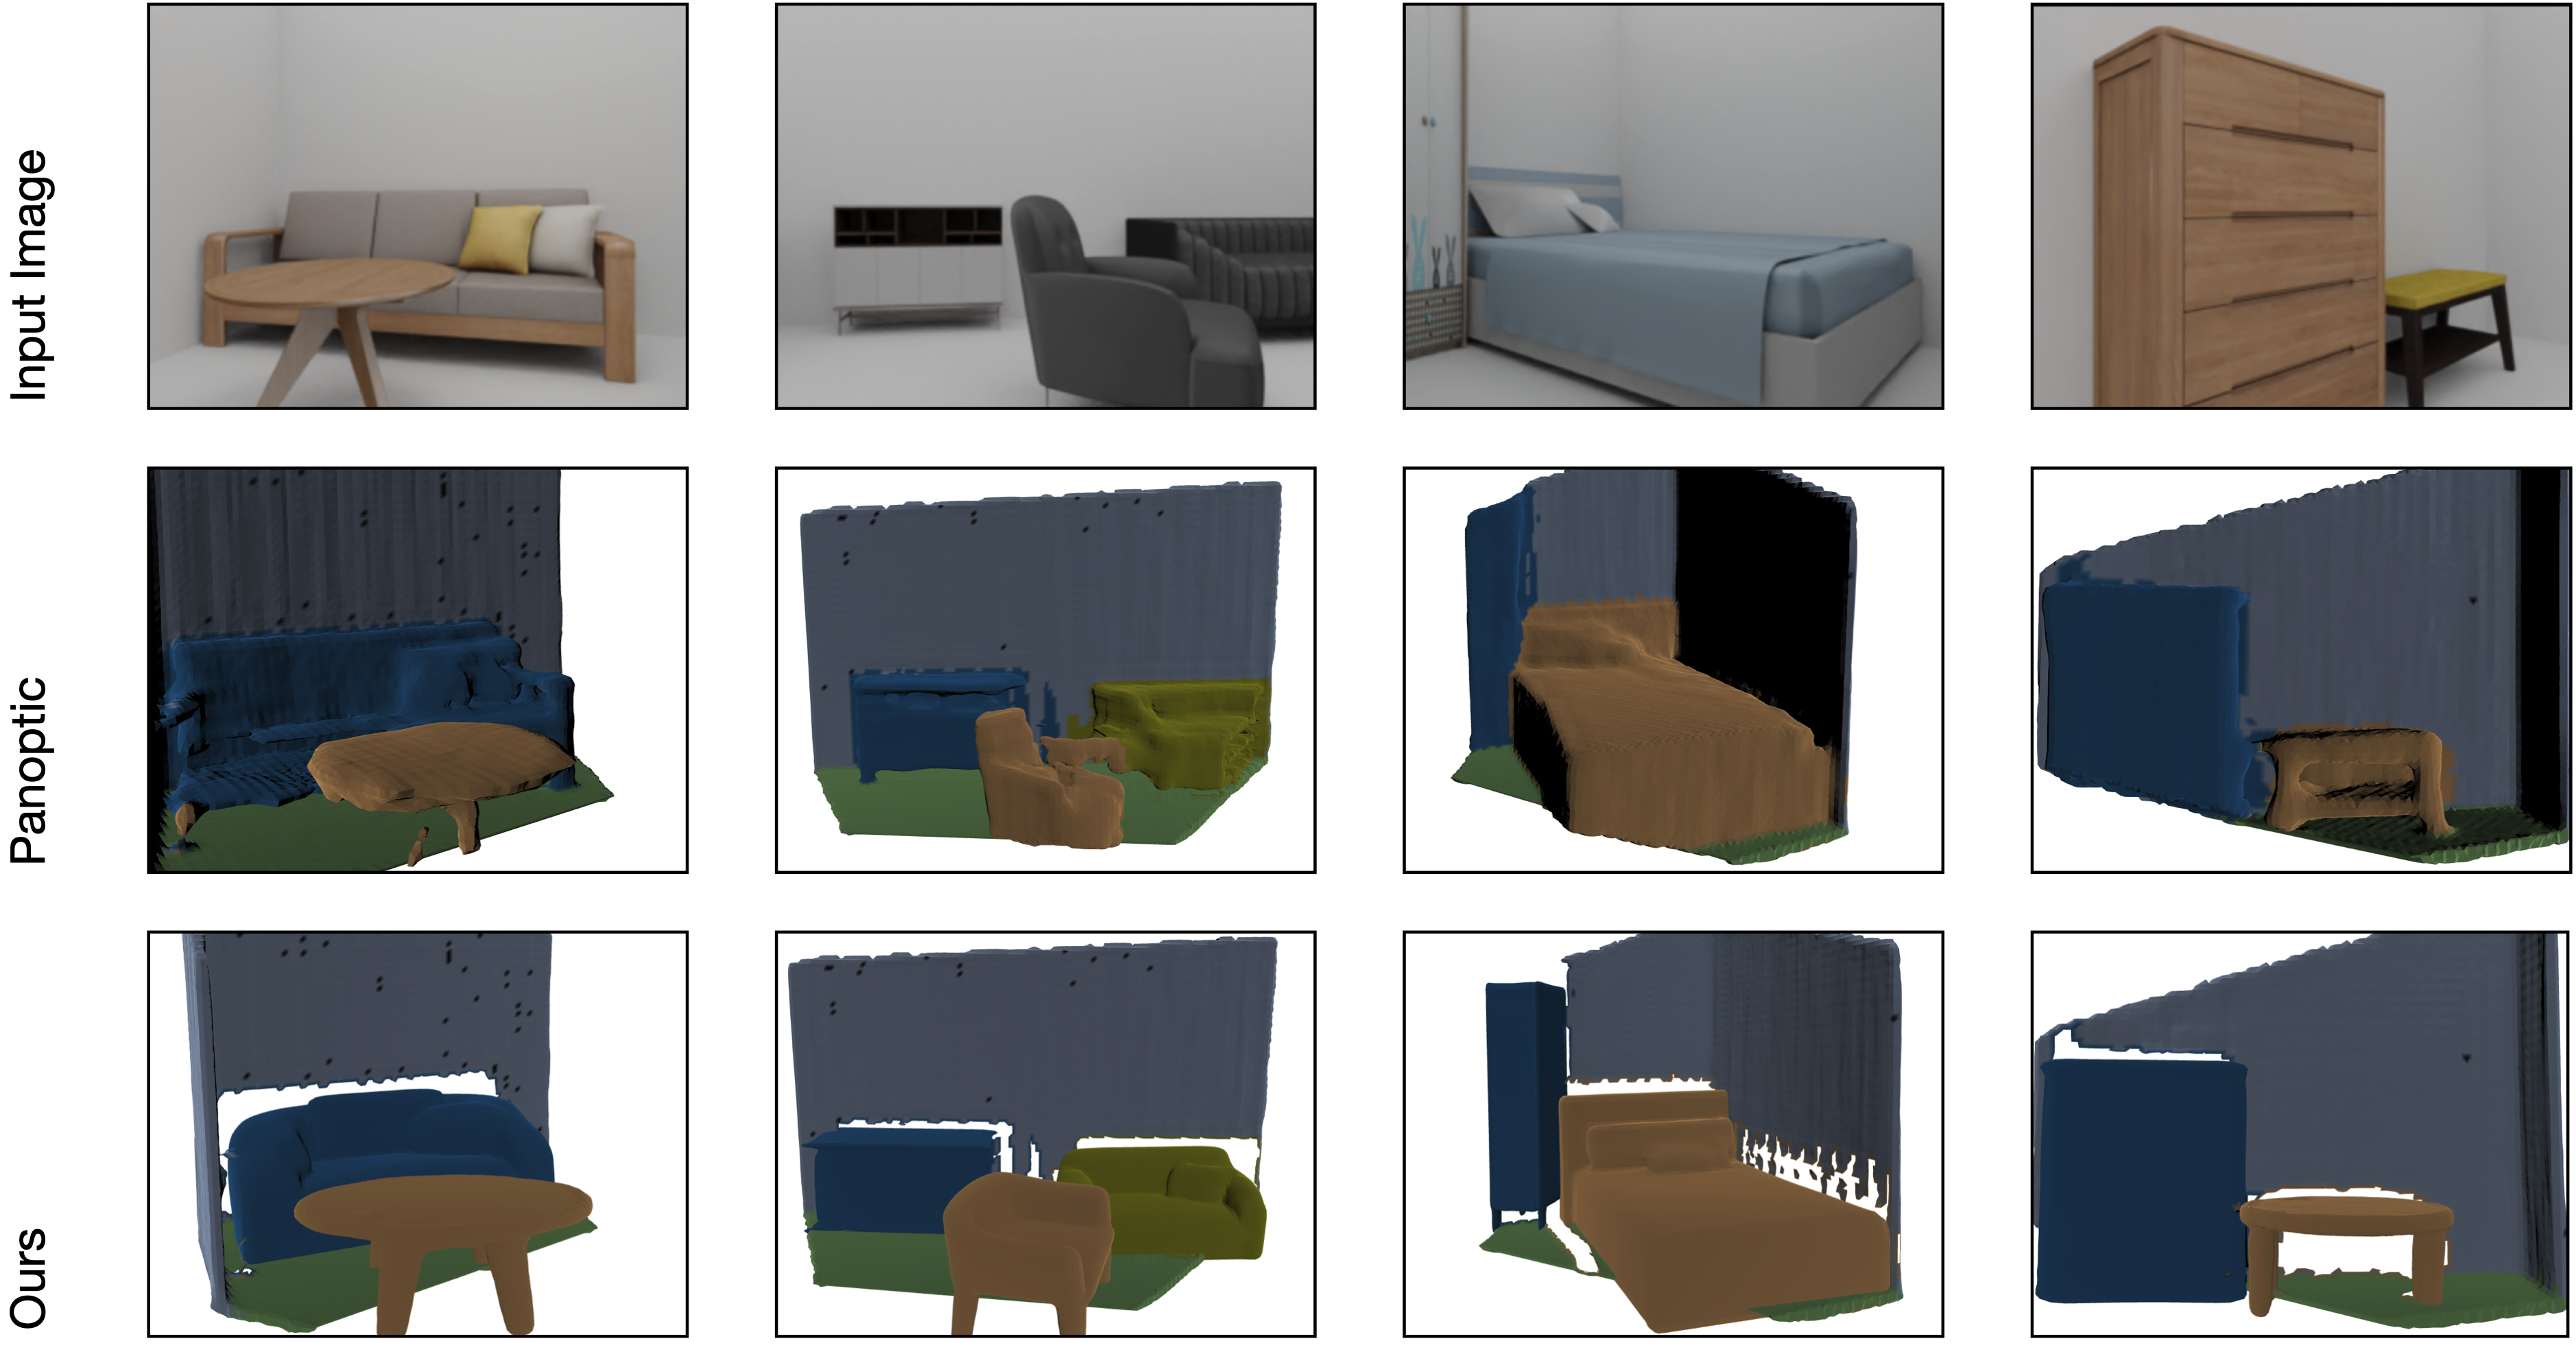
\includegraphics[width=\linewidth]{images/image1.png}
    \caption{While panoptic reconstruction fails to reconstruct unobserved regions, resulting in artifacts and missing geometry, our method successfully generates complete and distinguishable 3D geometry for each instance.}\label{fig:comparison_good}
  \end{subfigure}
  \qquad
  \begin{subfigure}[t]{56mm}
    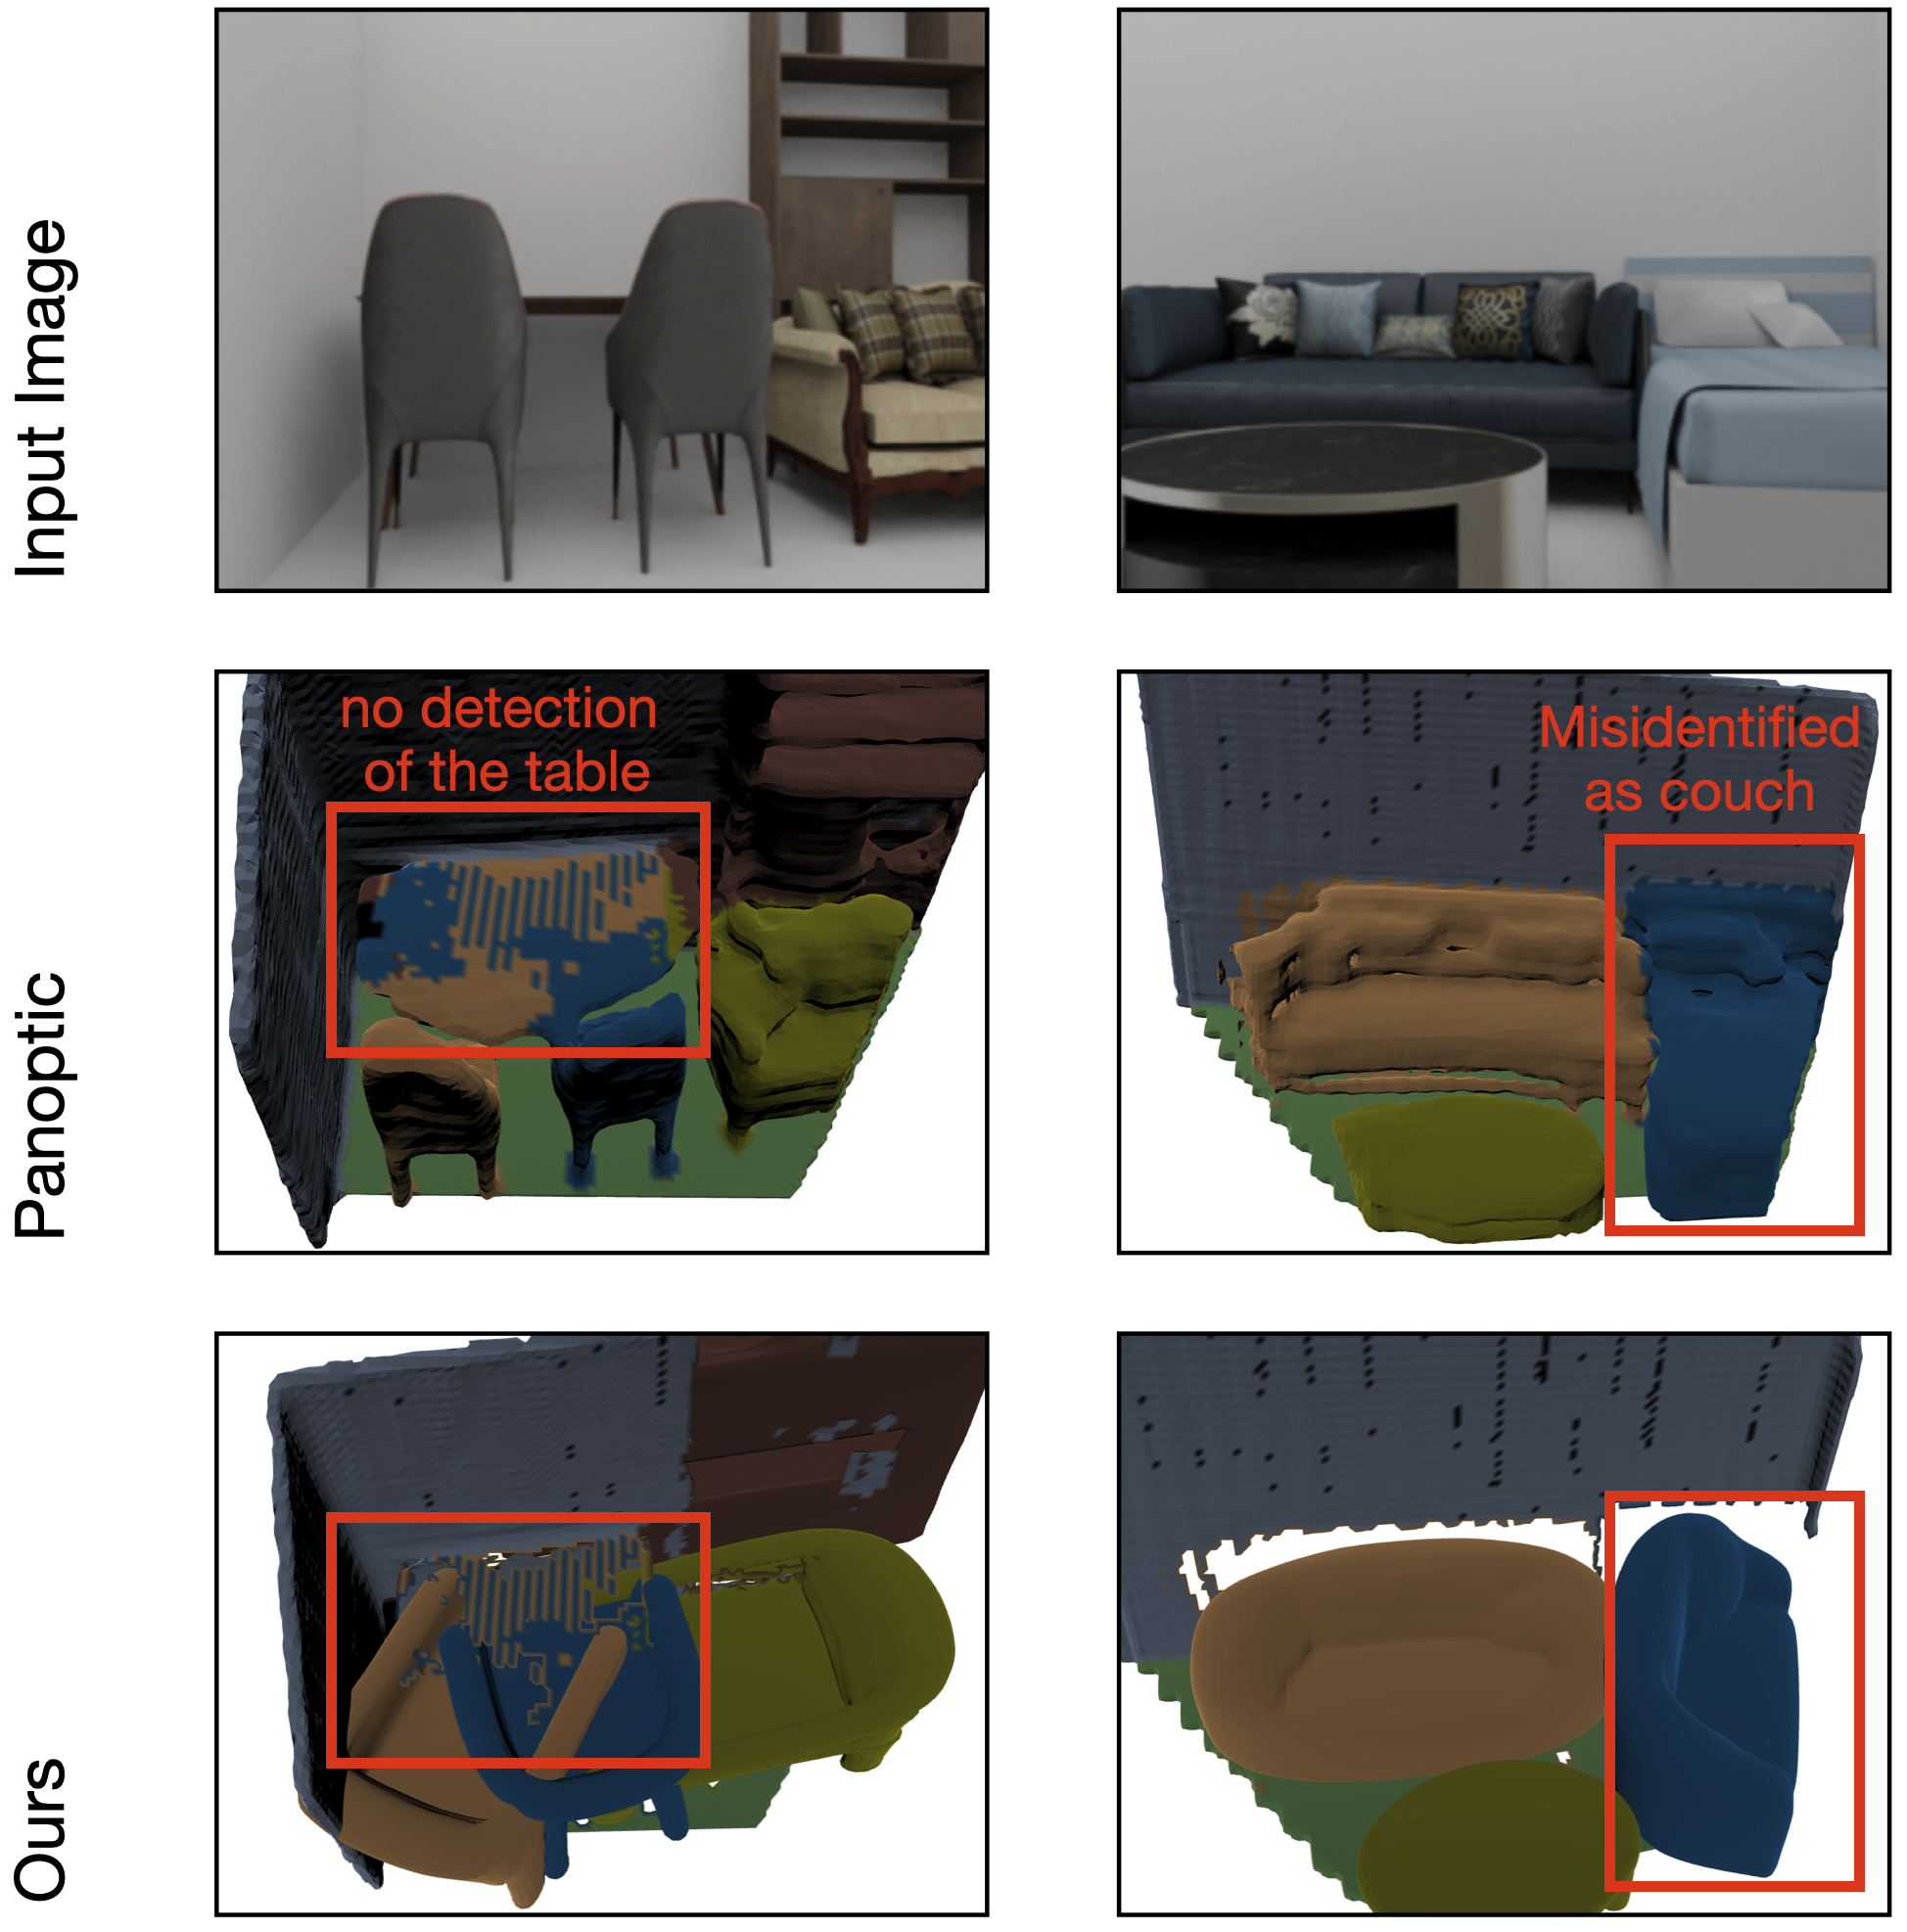
\includegraphics[width=\linewidth]{images/image2.png}
    \caption{We showcase scenarios in which our method encounters challenges in scene reconstruction. On the left, a scene is depicted where our method struggles due to missing instances, while on the right, an object is misclassified, resulting in an erroneous reconstruction.}\label{fig:comparison_bad}
  \end{subfigure}
  \caption{Comparison of panoptic vs ours}
  \label{fig:comparison_all}
\end{figure*}

The comparison between reconstructed scenes generated by our method and those produced by panoptic reconstruction is illustrated in \ref{fig:comparison_good}.
The panoptic reconstruction results exhibit instances that are noisy and lack clear edges from neighboring geometries.
Additionally, unobserved areas, whether occluded by other objects or out of sight, are disregarded, resulting in incomplete geometries within the reconstructed scene.
In \ref{fig:comparison_bad}, artifacts introduced by panoptic reconstruction for unobserved regions are highlighted.
In contrast, our method enhances all three properties: instances are clean, distinct from surrounding geometries, and represented as complete objects.
This improvement can be attributed to SDFusion's diffusion model, which effectively generates complete shapes from occluded SDF inputs, text, or images alone.
Moreover, our approach treats each object separately in SDFusion, resulting in distinct object geometries by design. The merging process in our method also ensures proper placement of refined instances within the scene.


\paragraph{SDFusion Fine-tuning}
In order to align SDFusion to the shape distribution of 3D-Front, we fine-tune the model on a subset of the 3D-Future dataset \citep{fu20213e}, which contains the objects used in the scenes of 3D-Front.
We train the model for 12k steps using the original hyperparameters from \citet{cheng2023sdfusion} but with a batch size of 32 (see Figure \ref{fig:finetune}).

\begin{figure}
  \centering
  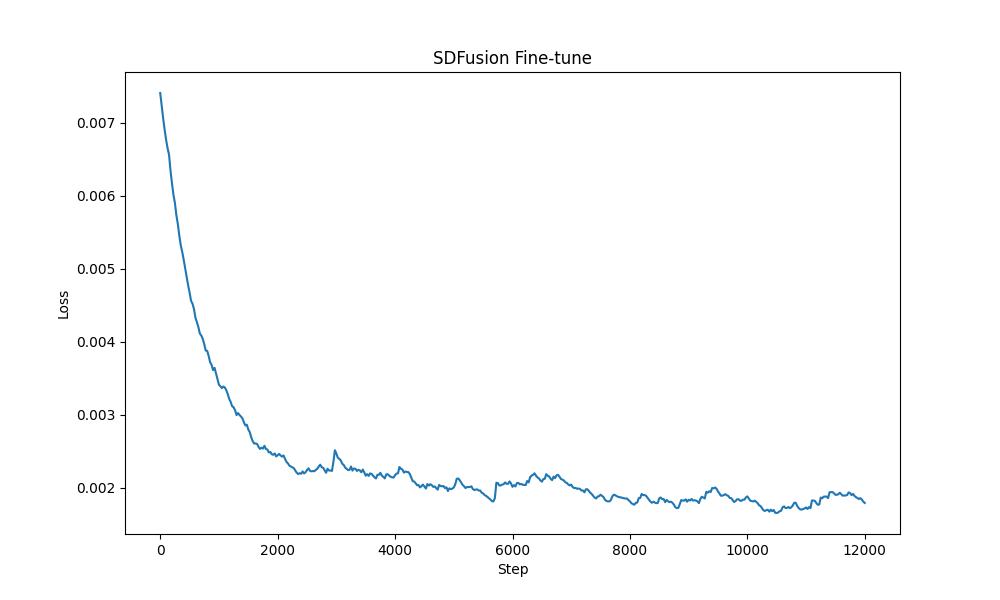
\includegraphics[width=\linewidth]{figs/sdfusion_finetune_loss_plot.png}
  \caption{Loss curve of our SDFusion fine-tune (smoothed).}
  \label{fig:finetune}
\end{figure}

\begin{figure}[H]
  \centering
  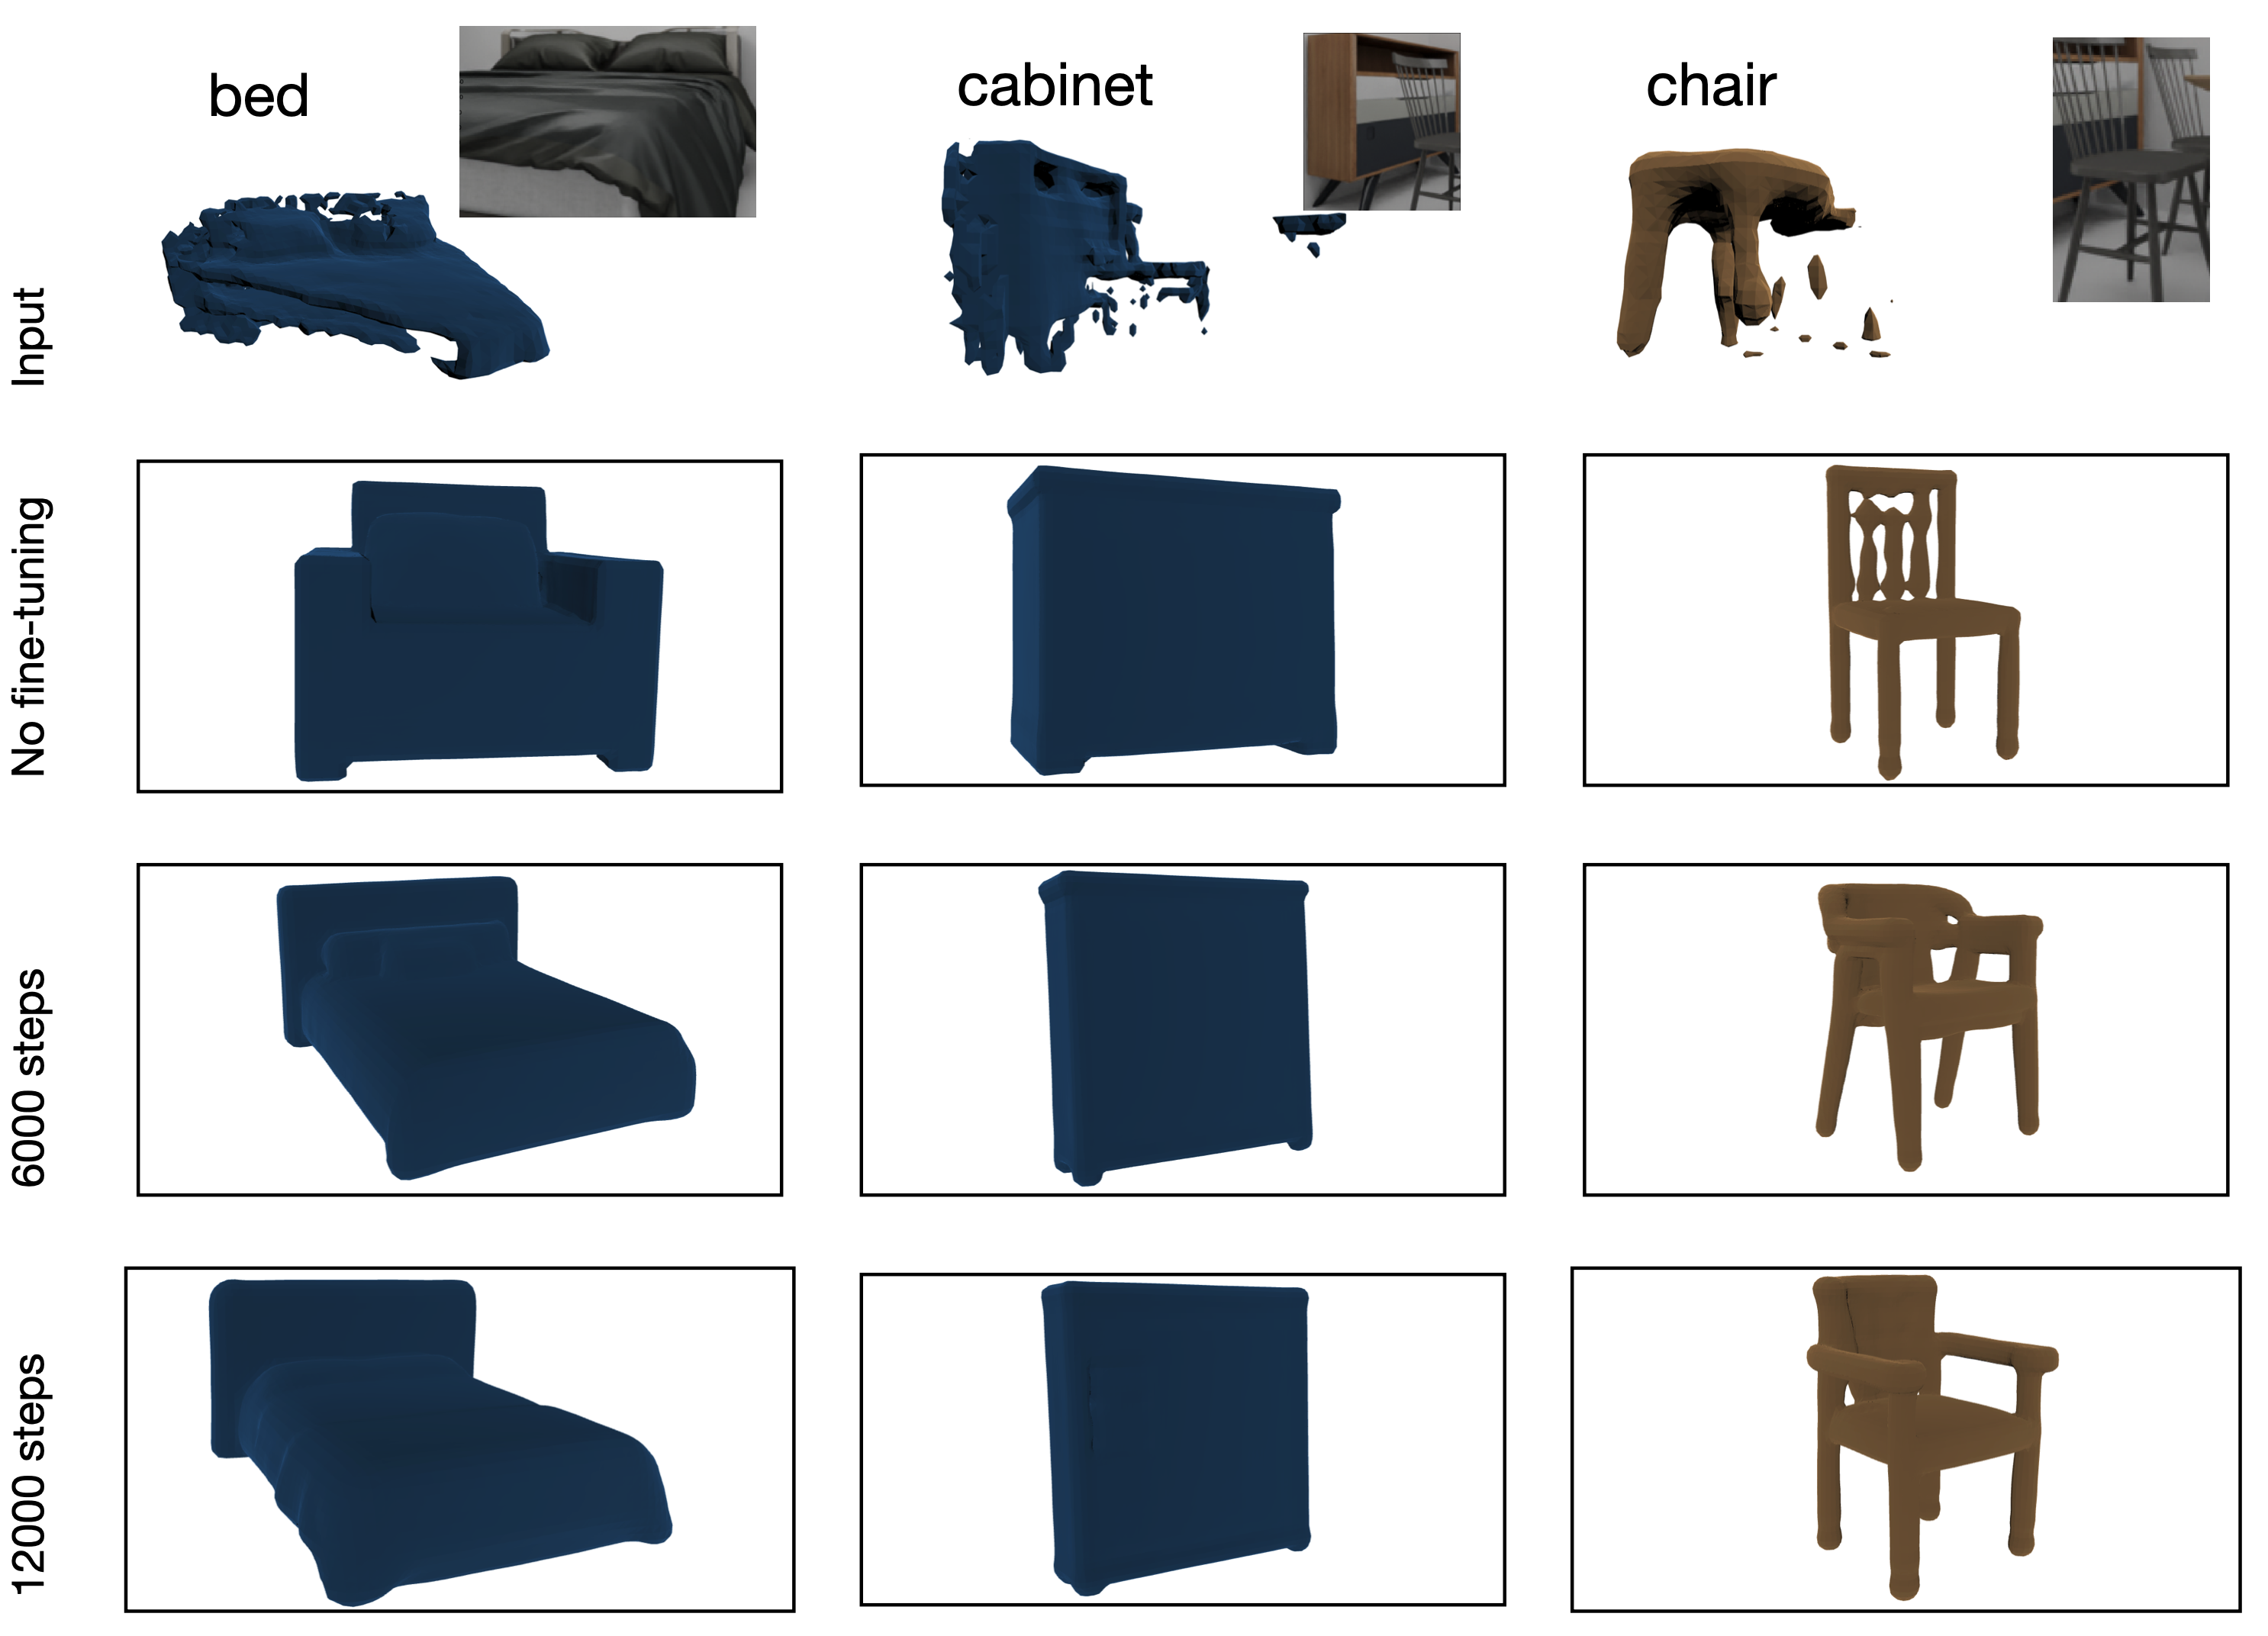
\includegraphics[width=80mm, scale=1]{images/image4.png}
  \caption{Fine-tuning results for SDFusion}
\end{figure}
